%# -*- coding: utf-8-unix -*-
% !TEX program = xelatex
% !TEX root = ../thesis.tex
% !TEX encoding = UTF-8 Unicode
%%==================================================
%% chapter02.tex for SJTU Master Thesis
%% based on CASthesis
%% modified by wei.jianwen@gmail.com
%% Encoding: UTF-8
%%==================================================

\chapter{决策与规划}
\label{chap:chapter04}


\section{路径规划}
\label{sec:pathplanning}
\subsection{航道保持}
航道保持算法是无人船默认的局部路径规划算法, 其适用于中高速航行的船舶,同时可实现多种规划目标
(例如速度保持、超越、跟踪和停止等)。
\subsubsection{Jerk}
\begin{theorem}
\label{thm:jerktheorem}
给定初始时刻$t_0$的初始状态$P_0=[p_0, \dot{p}_0,\ddot{p}_0]$以及结束时刻$t_1= t_0+T$
的状态$P_1=[ \dot{p}_1,\ddot{p}_1]$, 五次多项式是下列惩罚函数的最优解,
\begin{equation}
  \begin{aligned}
    &C=k_j J_t + k_t g(T) + k_p h(p_1) \\
    &J_t(p(t)):=\int_{t_0}^{t_1} \dddot{p}^2(\tau) d \tau
  \end{aligned}
\end{equation}
其中,$g$和$h$是任意函数,$k_j, k_t, k_p>0$, $J_t$(Jerk)通常用于描述加加速度的积分,
其与交通工具的舒适程度有关。
\end{theorem}

\subsubsection{Frenet坐标系}
Frenet坐标系被广泛用于轨迹跟踪和轨迹生成算法中\cite{werling2010optimal}。
在Frenet坐标系中(见图\ref{fig:trajectoryfrenet}),我们以参考轨迹点为原点建立参考坐标系$(\bm{t}_r, \bm{n}_r)$,生成的轨迹点$\bm{x}(s(t),d(t))$可表示为
\begin{equation}
  \label{eq:frenetcoordinate}
  \bm{x}(s(t),d(t)) = \bm{r}(s(t)) + d(t) \cdot \bm{n_r}(s(t))
\end{equation}
表\ref{tab:frenetsymbol}列出了常用的符号,同时我们定义$\dot{(\cdot)}:=
\frac{\partial}{\partial t}(\cdot)$和$(\cdot)':=
\frac{\partial}{\partial s}(\cdot)$

\begin{table}[htbp]
  \centering
  \caption{符号解释}
    \begin{tabular}{ll}
    \toprule
    符号    & 物理含义 \\
    \midrule
    $t$          & 时间 \\
    $T$          & 时间间隔 \\
    $\bm{r}$     & 移动参考坐标系原点(即参考轨迹点)的笛卡尔坐标 \\
    $s$          & 参考轨迹点的弧坐标 \\
    $d$          & 生成轨迹点相对于参考轨迹点的横向偏移量 \\
    $\bm{t}_r$   & 移动参考坐标系的切向量 \\
    $\bm{n}_r$   & 移动参考坐标系的法向量 \\
    $\bm{t}_x$   & 生成轨迹点的切向量 \\
    $\bm{n}_x$   & 生成轨迹点的切向量 \\
    $\bm{x}$     & 生成轨迹的笛卡尔坐标 \\
    $\theta_r$   & 参考轨迹点的方向角 \\
    $\kappa_r$   & 参考轨迹点的曲率 \\
    $\theta_x$   & 生成轨迹点的方向角 \\
    $\kappa_x$   & 生成轨迹点的曲率 \\
    $v_x$  & 生成轨迹点的速度大小 \\
    $a_x$  & 生成轨迹点的加速度大小 \\
    \bottomrule
    \end{tabular}%
  \label{tab:frenetsymbol}%
\end{table}%

\begin{figure}[!htp]
  \centering
  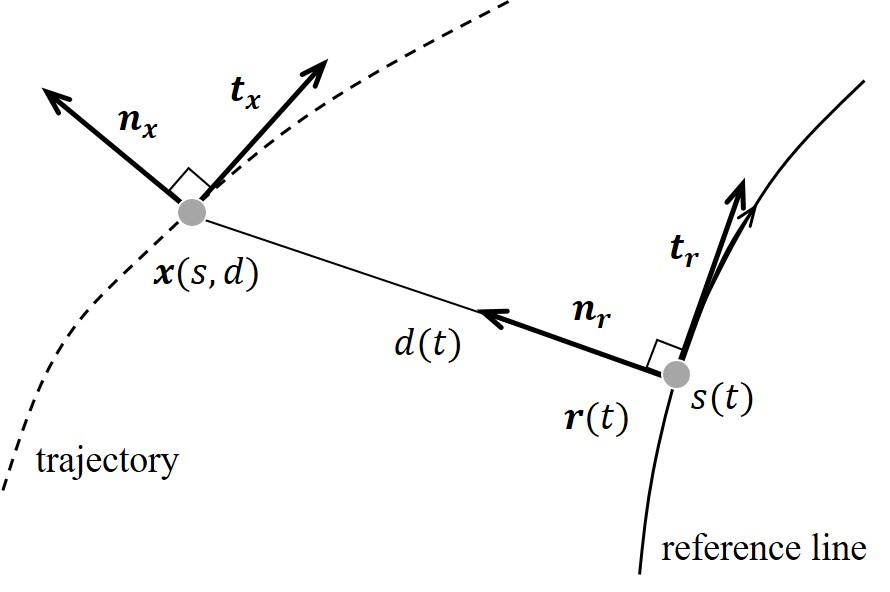
\includegraphics[width=10cm]{chapter04/trajectoryfrenet.jpg}
  \bicaption[Frenet坐标系下的轨迹生成]
    {Frenet坐标系下的轨迹生成}
    {Trajectory generation in a Frenet frame}
  \label{fig:trajectoryfrenet}
\end{figure}

\subsubsection{横向轨迹规划}
\begin{itemize}
  \item \textbf{中高速}

  给定横向的初始状态$D_0=[d_0, \dot{d}_0, \ddot{d}_0]$, 我们假设$\dot{d}_1=\ddot{d}_1=0$
  (这也是我们期望的最终状态),并假设$g(T)=T, \quad h(d_1)=d_1^2$, 由此可得
  \begin{equation}
    C_d = k_j J_t(d(t))+k_t T + k_d d_1^2
  \end{equation}
  $C_d$中最后一项用于惩罚最终状态$d \neq 0$的情况。由定理\ref{thm:jerktheorem}可得,
  $d(t)$是关于$t$的五次多项式(quintic polynomials)。通过调整最终状态的$d_i$和$T_j$
  \begin{equation}
    [d_1,\dot{d}_1,\ddot{d}_1,T]_{ij}=[d_i,0,0,T_j]
  \end{equation}
  注意,船体的状态是实时变化的,因此$D_0$始终表示船体当前时刻的状态,相应的$D_1$表示规划的
  最终状态,也是实时变化的。

  \item \textbf{低速}

  对于中高速的情况下,$s(t)$和$d(t)$可以被分开计算;但对于低速的情况,对$s(t)$和$d(t)$
  独立处理的方法违背了刚体运动的non-holonomic的性质,因此横向轨迹的计算需要考虑纵向轨迹
  \begin{equation}
    \bm{x}(s(t),d(t)) = \bm{r}(s(t)) + d(s(t)) \cdot \bm{n}_r(s(t))
  \end{equation}
  考虑低速的情形,我们修改了惩罚函数
  \begin{equation}
    \begin{aligned}
      &C_d = k_j J_s(d(s)) + k_t S + k_d d_1^2 \\
      &J_s(d(s)):= \int_{s_0}^{s_1} d'''^2(\sigma) d \sigma
    \end{aligned}
  \end{equation}
  该惩罚函数的最优值是$d(s)$关于$s$的五次多项式,且该多项式的初始点$D_0=[d_0, d'_0, d''_0]$
  和终止点为
  \begin{equation}
    [d_1, d'_1,d''_1, T]_{ij}=[d_i, 0, 0, T_j]
  \end{equation}
\end{itemize}

\subsubsection{纵向轨迹规划}
对于纵向的轨迹规划,主要分为跟踪、超越、速度保持和停止。
\begin{itemize}
  \item \textbf{速度保持}

  未感知到障碍物的时候,我们希望船舶匀速航行。结合$s_1$的Transversality condition
  \cite{IROS637936}和定理\ref{thm:jerktheorem},可知四次多项式(quartic polynomials)能够
  使得以下惩罚函数最小,
  \begin{equation}
    C_v = k_j J_t(s(t)) + k_t T + k_{\dot{s}}[\dot{s}_1-\dot{s}_d]^2
  \end{equation}
  其中,我们给定$t_0$时刻$S_0=[s_0, \dot{s}_0, \ddot{s}_0]$,$t_1=t_0+T$时刻的状态
  $S_1=[\dot{s}_1,\ddot{s}_1]$。这就意味着,$s$可以用$t$的四次多项式表示,而多项式的
  初始条件分别为$S_0=[s_0, \dot{s}_0, \ddot{s}_0]$和以下终止条件
  \begin{equation}
    [\dot{s}_1, \ddot{s}_1, T]_{ij}= [\dot{s}_d+\Delta \dot{s}_i, 0, T_j]
  \end{equation}
  当我们调整$\Delta \dot{s}_i$和$T_j$时,可得不同终止条件下的轨迹。
  \item \textbf{跟踪}

  对于跟踪、超越和停止的情况,都存在目标的位置$s_{target}(t)$,给定了$S_0 = [s_0,
  \dot{s}_0, \ddot{s}_0]$和以下的终止条件
  \begin{equation}
    [s_1, \dot{s}_1,\ddot{s}_1, T]_{ij}=[s_{target}(T_j)+\Delta s_i \: ,
    \dot{s}_{target}(T_j) \: , \ddot{s}_{target}(T_j) \: , T_j]
  \end{equation}
  可得$s(t)$关于$t$的五次多项式是以下惩罚函数(cost function)的最优解,
  \begin{equation}
    C_t = k_j J_t + k_t T + k_s(s_1-s_d)^2
  \end{equation}
  当我们调整终止条件中的$\Delta s_i$和$T_j$,可得多条纵向轨迹。

  对于跟踪,也就是与前方的船舶保持一定的距离,这个距离也需要满足海事规范,
  \begin{equation}
    s_{target}(t):=s_{lv}(t)-(D_0+\tau \dot{s}_{lv}(t))
  \end{equation}
  其中,$D_0$和$\tau$是常数,$s_{lv}$和$\dot{s}_{lv}$分别是领导船只沿轨迹线的位置和速度。
  \item \textbf{超越和停止}

  \begin{equation}
    s_{target}(t)=\frac{1}{2}[s_a(t)+s_b(t)]
  \end{equation}
  其中$s_a(t)$和$s_b(t)$分别是周围两条船的位置。对于停止的情况,
  $s_{target}=s_{stop} \, , \, \dot{s}_{target}=0 \, , \, \ddot{s}_{target}=0$
\end{itemize}

\subsubsection{轨迹结合}
通过调整终止条件,我们可得横向和纵向的多项式线束(Lattice),$\Pi_{lat}$和$\Pi_{lon}$,
从而生成轨迹线束$\Pi_{lat} \times \Pi_{lon}$,如图\ref{fig:frenetlattice}所示。在选取
最优轨迹的过程中,我们考虑联合惩罚函数$C_{tot}=k_{lat}C_{lat}+k_{lon}C_{lon}$, 同时保证
生成轨迹与障碍物有一定的安全距离。最终保证避障的条件下,选取最优轨迹。

\begin{figure}[!htp]
  \centering
  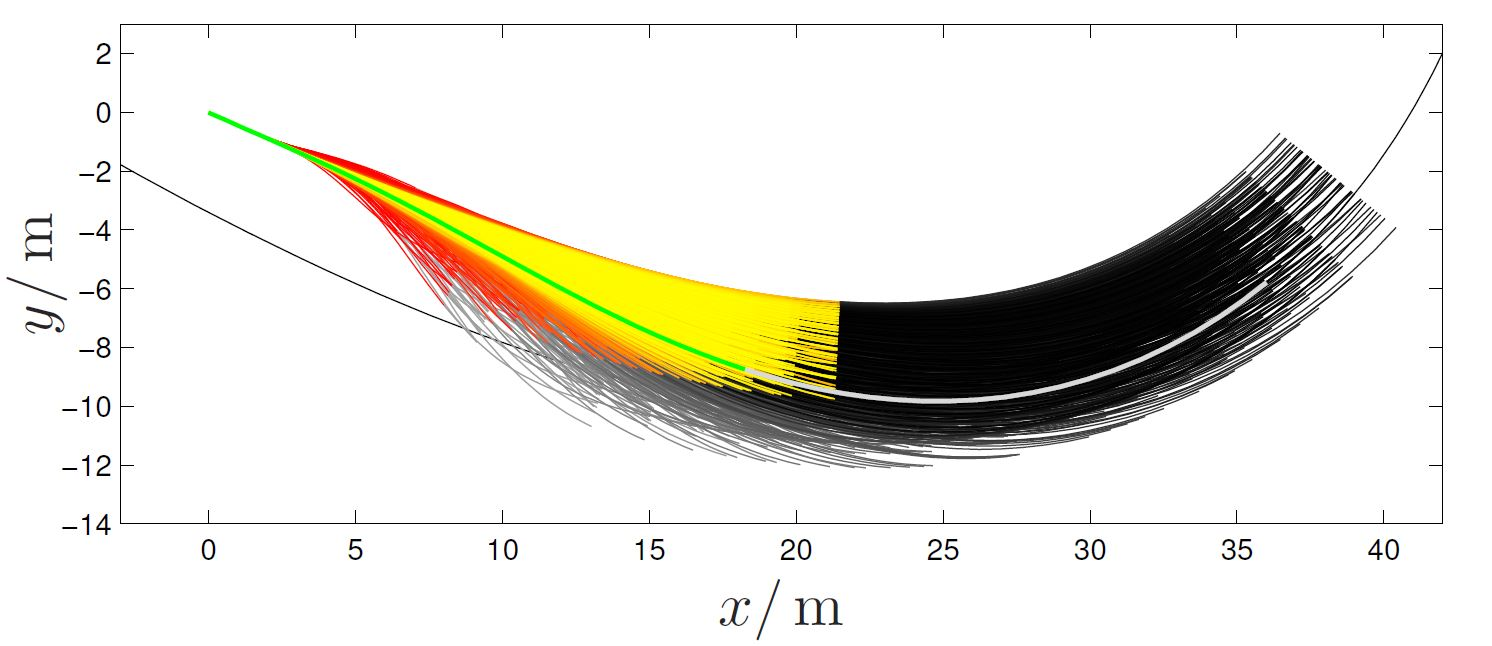
\includegraphics[width=12cm]{chapter04/frenetlattice.jpg}
  \bicaption[Frenet坐标系下的最优轨迹线束]
    {Frenet坐标系下的最优轨迹线束, 其预测时间为3秒,红色到黄色代表递增的惩罚值(cost),
    当障碍物不存在时,“绿-灰”的轨迹即为最优轨迹,使得船体回归参考轨迹。}
    {Resulting trajectory set in global coordinates for velocity keeping: The color map visualizes the increasing costs of both the reactive layer with 3.0 s lookahead from red to yellow and the alternatives for the long-term objectives form gray to black. As there are no obstacles within the 3.0 s horizon, the optimal trajectory of the free problem is chosen (green, light gray), which leads the vehicle back to the center line and to the desired speed.
    }
  \label{fig:frenetlattice}
\end{figure}


\subsubsection{坐标转换}
计算轨迹线束时,需要Frenet坐标系和Cartesian坐标系的相互转换。Frenet坐标系下的船体状态为
$ [s, \dot{s}, \ddot{s} \,; d, \dot{d},\ddot{d}/d, d', d'']$和$[\bm{x}, \theta_x, \kappa_x, v_x, a_x]$,首先我们推导一些通用的公式。

我们定义$\bm{t}_r(s):=[\cos(\theta_r(s)) \: \sin(\theta_r(s))]^T$,
$\bm{n}_r(s):=[ -\sin(\theta_r(s)) \: \cos(\theta_r(s))]^T$和
$\Delta \theta:=\theta_x - \theta_r$,且确保$|\Delta \theta| < \frac{\pi}{2}$和
$1-\kappa_r d >0$。
由Frenet-Serret公式可得
\begin{equation}
  \begin{aligned}
    &\frac{\mathrm{d} \bm{n}_r}{\mathrm{d} s} = -{\kappa}_r \bm{t}_r, \quad
    \frac{\mathrm{d} \bm{n}_r}{\mathrm{d} t} = -\dot{s}{\kappa}_r \bm{t}_r \\
    &\frac{\mathrm{d} \bm{t}_r}{\mathrm{d} s} = {\kappa}_r \bm{n}_r, \quad
    \frac{\mathrm{d} \bm{t}_r}{\mathrm{d} t} = \dot{s} {\kappa}_r \bm{n}_r
  \end{aligned}
\end{equation}
结合Frenet-Serret公式,由方程\ref{eq:frenetcoordinate}可得
\begin{equation}
  d=[\bm{x}-\bm{r}(s)]^T \cdot \bm{n}_r
\end{equation}
对上式作时间的导数,可得
\begin{equation}
  \begin{aligned}
    \dot{d}
    &=[\dot{\bm{x}}-\dot{\bm{r}}(s)]^T \bm{n}_r +
            [\bm{x}-\bm{r}(s)]^T \dot{\bm{n}}_r \\
    &=v_x \bm{t}_x^T \bm{n}_r - \dot{s} \bm{t}_r^T \bm{n}_r - \dot{s} {\kappa}_r
    [\bm{x}-\bm{r}(s)]^T \bm{t}_r \\
    &= v_x \sin(\Delta \theta)
  \end{aligned}
\end{equation}
同时,我们得到
\begin{equation}
  \begin{aligned}
    v_x
    &= || \dot{\bm{x}} ||_2 \\
    &= || \dot{\bm{r}}(s) + \dot{d} \bm{n}_r +d \dot{\bm{n}}_r ||_2 \\
    &= || \dot{s}\bm{t}_r + \dot{d} \bm{n}_r - \dot{s} {\kappa}_r d \bm{t}_r ||_2 \\
    &= \left\|
        \left[
          \begin{array}{cc}
            {\bm{t}_{r}} & {\bm{n}_{r}}
          \end{array}
        \right]
        \left[
          \begin{array}{cc}
            {1-\kappa_{r} d} & {0} \\ {0} & {1}
          \end{array}
        \right]
        \left[
          \begin{array}{c}
            {\dot{s}} \\ {\dot{d}}
          \end{array}
        \right]
      \right\|_2 \\
    &= \sqrt{(1-{\kappa}_r d)^2 \dot{s}^2 +\dot{d}^2}
  \end{aligned}
\end{equation}
且
\begin{equation}
  \label{eq:ddds}
  \begin{aligned}
    d'
    &=\frac{\mathrm{d} t}{\mathrm{d} s} \frac{\mathrm{d} }{\mathrm{d} t} d
    =\frac{\dot{d}}{\dot{s}} = \frac{1}{\dot{s}} v_x \sin(\Delta \theta) \\
    &=\sqrt{(1-{\kappa}_r d)^2 +d'^2}  \sin(\Delta \theta) \\
    & \Rightarrow \\
    d'
    &=(1-{\kappa}_rd) \tan(\Delta \theta)
  \end{aligned}
\end{equation}
已知$(\bm{x}-\bm{r}(s))^T \bm{t}_r = 0$,对其作时间导数可得 $  \frac{v_x}{\dot{s}} \cos(\Delta \theta) -1 + {\kappa}_r d = 0$, 变化得到船体的速度大小
\begin{equation}
  v_x = \dot{s} \frac{1-{\kappa}_r d}{\cos(\Delta \theta)}
\end{equation}
我们用$s_x$表示轨迹$\bm{x}$上的弧长,根据曲率的定义${\kappa_x}=\frac{\mathrm{d} \theta_x}{\mathrm{d}s_x}$和${\kappa_r}=\frac{\mathrm{d} \theta_r}{\mathrm{d}s}$,
可得
\begin{equation}
  \frac{\mathrm{d}}{\mathrm{d}s} =\frac{\mathrm{d} s_x}{\mathrm{d}t}
  \frac{\mathrm{d} t}{\mathrm{d} s} \frac{\mathrm{d}}{\mathrm{d}s_x}
  = \frac{v_x}{\dot{s}} \frac{\mathrm{d}}{\mathrm{d}s_x}
  =\frac{1-{\kappa}_r d}{\cos(\Delta \theta)} \frac{\mathrm{d}}{\mathrm{d}s_x}
\end{equation}
\begin{equation}
  \begin{aligned}
    \Delta \theta ' = \frac{\mathrm{d}( {\theta}_x - {\theta}_r)}{\mathrm{d}s}
    &= \frac{\mathrm{d}}{\mathrm{d} s} {\theta}_x - {\kappa}_r \\
    &= \frac{1-{\kappa}_r d}{\cos(\Delta \theta)} {\kappa}_x - {\kappa}_r  \\
  \end{aligned}
\end{equation}
由公式\ref{eq:ddds},我们可得$d$对$s$的二阶导数
\begin{equation}
  d''=-({\kappa}_r  d)' \tan(\Delta \theta) + \frac{1-{\kappa}_r d}
  {\cos^2(\Delta \theta)}    \Delta \theta '
\end{equation}
将速度$v_x$对时间求导可得
\begin{equation}
  a_x := \dot{v}_x = \ddot{s}\frac{1-{\kappa}_r d}{\cos(\Delta \theta)}  +
  \frac{\dot{s}^2}{\cos(\Delta \theta)}[d' \Delta \theta' - ({\kappa}_r d)']
\end{equation}
同时, $s$对时间$t$的二阶导数
\begin{equation}
  \ddot{s}=\frac{a_x \cos(\Delta \theta)- \dot{s}^2
  [d' \Delta \theta' - ({\kappa}_r d)']}{1-{\kappa}_r d}
\end{equation}
在中高速的情况下($d$与$s$无关),
\begin{equation}
  \begin{aligned}
    &\dot{d}=\frac{\mathrm{d}}{\mathrm{d} t}d=\frac{\mathrm{d}s}{\mathrm{d} t}
    \frac{\mathrm{d}}{\mathrm{d} s}d= \dot{s}d' \\
    &\ddot{d}=d'' \dot{s}^2 + d' \ddot{s}
  \end{aligned}
\end{equation}


坐标系之间的转换将会用于Frenet Lattice的实时计算中(如图\ref{fig:frenetalgorithm}),
下面我们分别讨论两个坐标系之间的转换过程
\begin{itemize}
  \item \textbf{从Cartesian到Frenet}

  给定船体当前时刻的状态为$[\bm{x},\theta_x, \kappa_x, v_x, a_x](t_0)$, 我们希望得到
  在Frenet坐标系下,当前时刻的状态$[s_0, \dot{s}_0, \ddot{s}_0, d_0, \dot{d}_0,
  \ddot{d}_0]$或者$[s_0, \dot{s}_0, \ddot{s}_0, d_0, d'_0, d''_0]$。
  \begin{equation}
    [\bm{x}, \theta_x, \kappa_x, v_x, a_x]  \rightarrow
    [s, \dot{s}, \ddot{s}; d, \dot{d},\ddot{d}/d, d', d'']
  \end{equation}
  首先,采用一些高效的数值方法得到船体在参考轨迹上的投影点$s$
  \begin{equation}
    s= arg\,min_{\sigma} || \bm{x}-\bm{r}(\sigma)||
  \end{equation}
  得到$s$之后,根据参考轨迹的多项式公式,可得${\kappa}_r, {\kappa}'_r$和${\theta}_r$,
  从而计算$\Delta \theta = {\theta}_x-{\theta}_r $, 剩下的变量也可以根据以上公式推导
  得到。

  \item \textbf{从Frenet到Cartesian}

  当我们得到生成轨迹$[s, \dot{s}, \ddot{s}; d, \dot{d},\ddot{d}/d, d', d'']$的时候,
  需要得出Cartesian坐标系中,生成轨迹的状态
  \begin{equation}
    [s, \dot{s}, \ddot{s}; d, \dot{d},\ddot{d}/d, d', d''] \rightarrow
    [\bm{x}, \theta_x, \kappa_x, v_x, a_x]
  \end{equation}

\end{itemize}


\begin{figure}[!htp]
  \centering
  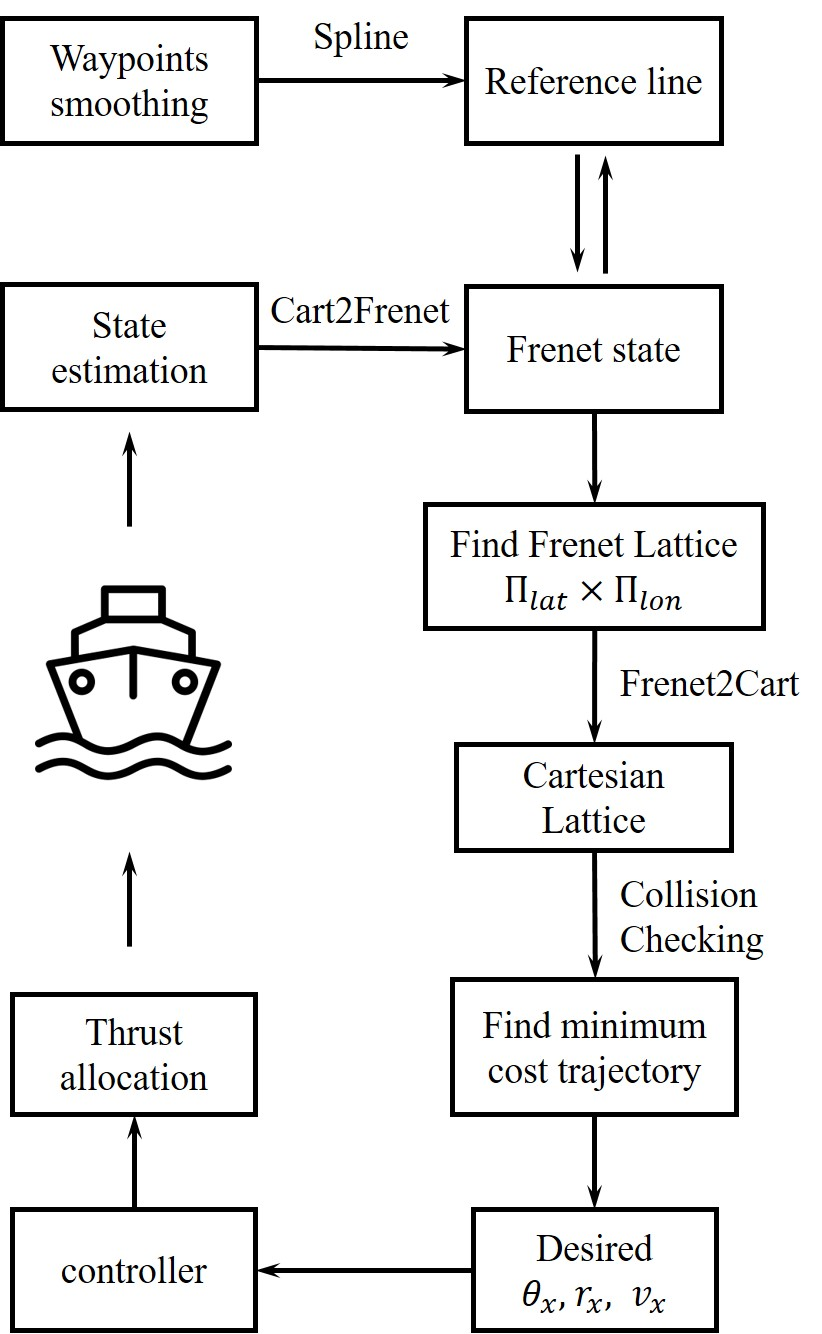
\includegraphics[width=9cm]{chapter04/Algorithm.jpg}
  \bicaption[Frenet坐标系下的最优轨迹生成算法逻辑图]
    {Frenet坐标系下的最优轨迹生成算法逻辑图}
    {Flowchart for trajectory generator in the Frenet frame}
  \label{fig:frenetalgorithm}
\end{figure}


\subsection{低速泊船}
Hybrid A Star algorithm


\section{航线规划}
\label{sec:routeplanning}


\section{行为规划}
\label{sec:behav}
